\chapter{Implementacija i korisničko sučelje}
		
		\section{Korištene tehnologije i alati}
		
			Komunikacija u timu realizirana je korištenjem aplikacija \underline{WhatsApp}\footnote{https://www.whatsapp.com/} i \underline{Discord} \footnote{https://discord.com/}. Za izradu	UML dijagrama korišten je alat \underline{Astah UML} \footnote{https://astah.net/products/astah-uml/}  , a kao sustav za upravljanje izvornim kodom \underline{Git}\footnote{https://git-scm.com/}. Udaljeni repozitorij projekta je dostupan na web platformi \underline{GitLab} \footnote{https://gitlab.com/} .
			Kao razvojno okruženje korišten je \underline{Visual Studio Code}\footnote{https://code.visualstudio.com/}. Prvenstveno se koristi kao uređivač teksta pri razvoju računalnih programa za operacijski sustav Windows, kao i za web-stranice, web-aplikacije, web-usluge i mobilne aplikacije. Aplikacija je napisana koristeći radni okvir \underline{Flask}\footnote{https://flask.palletsprojects.com/en/2.0.x/} i web poslužitelj \underline{Gunicorn}\footnote{https://gunicorn.org/} u jeziku \underline{Python 3.8}. \footnote{https://www.python.org/} za izradu backenda. Za izradu frontenda su se koristili razvojni okvir \underline{React}\footnote{https://reactjs.org/} i jezik \underline{JavaScript}\footnote{https://www.javascript.com/}. React, takoder poznat kao React.js ili ReactJS, je biblioteka u JavaScriptu za izgradnju korisničkih sučelja. React se najčešće koristi kao osnova	u razvoju web ili mobilnih aplikacija. Složene aplikacije u Reactu obično zahtijevaju korištenje dodatnih biblioteka za interakciju s API-jem. Web poslužitelj Gunicorn nadograđuje radni okvir Flask kako bi mogao posluživati više zahtjeva u isto vrijeme. Naša cijela infrastruktura se nalazi u oblaku na privatnom VPS poslužitelju, poslužuje zahtjeve pomoću \underline{NGINX}\footnote{https://nginx.org/en/} web poslužitelja na linux  ubuntu sustavu.
			Mrežna potpora našoj arhitekturi je \underline{CloudFlare} \footnote{https://www.cloudflare.com/} koja nam nudi usluge poput predmemorije (engl. cache) i DDoS zaštite. Bitan dio naše infrastrukture je baza podataka realizirana kroz \underline{PostgreSQL RDBMS}\footnote{https://www.postgresql.org/}.
			
			
			\eject 
		
	
		\section{Ispitivanje programskog rješenja}
			
			\textbf{\textit{dio 2. revizije}}\\
			
			 \textit{U ovom poglavlju je potrebno opisati provedbu ispitivanja implementiranih funkcionalnosti na razini komponenti i na razini cijelog sustava s prikazom odabranih ispitnih slučajeva. Studenti trebaju ispitati temeljnu funkcionalnost i rubne uvjete.}
	
			
			\subsection{Ispitivanje komponenti}
			\textit{Potrebno je provesti ispitivanje jedinica (engl. unit testing) nad razredima koji implementiraju temeljne funkcionalnosti. Razraditi \textbf{minimalno 6 ispitnih slučajeva} u kojima će se ispitati redovni slučajevi, rubni uvjeti te izazivanje pogreške (engl. exception throwing). Poželjno je stvoriti i ispitni slučaj koji koristi funkcionalnosti koje nisu implementirane. Potrebno je priložiti izvorni kôd svih ispitnih slučajeva te prikaz rezultata izvođenja ispita u razvojnom okruženju (prolaz/pad ispita). }
			
			
			
			\subsection{Ispitivanje sustava}
			
			 \textit{Potrebno je provesti i opisati ispitivanje sustava koristeći radni okvir Selenium\footnote{\url{https://www.seleniumhq.org/}}. Razraditi \textbf{minimalno 4 ispitna slučaja} u kojima će se ispitati redovni slučajevi, rubni uvjeti te poziv funkcionalnosti koja nije implementirana/izaziva pogrešku kako bi se vidjelo na koji način sustav reagira kada nešto nije u potpunosti ostvareno. Ispitni slučaj se treba sastojati od ulaza (npr. korisničko ime i lozinka), očekivanog izlaza ili rezultata, koraka ispitivanja i dobivenog izlaza ili rezultata.\\ }
			 
			 \textit{Izradu ispitnih slučajeva pomoću radnog okvira Selenium moguće je provesti pomoću jednog od sljedeća dva alata:}
			 \begin{itemize}
			 	\item \textit{dodatak za preglednik \textbf{Selenium IDE} - snimanje korisnikovih akcija radi automatskog ponavljanja ispita	}
			 	\item \textit{\textbf{Selenium WebDriver} - podrška za pisanje ispita u jezicima Java, C\#, PHP koristeći posebno programsko sučelje.}
			 \end{itemize}
		 	\textit{Detalji o korištenju alata Selenium bit će prikazani na posebnom predavanju tijekom semestra.}
			
			\eject 
		
		
		\section{Dijagram razmještaja}
			
			Dijagrami razmještaja opisuju topologiju sklopovlja i programsku potporu koja se koristi u implementaciji sustava u njegovom radnom okruženju. Na poslužiteljskom računalu se nalaze web poslužitelj i poslužitelj baze podataka. Klijenti koriste web preglednik kako bi pristupili web aplikaciji. Sustav je baziran na arhitekturi ”klijent – poslužitelj”, a komunikacija između računala korisnika (klijent, zaposlenik, vlasnik, administrator) i poslužitelja odvija se preko HTTPS veze.
			
			
			\begin{figure}[H]
				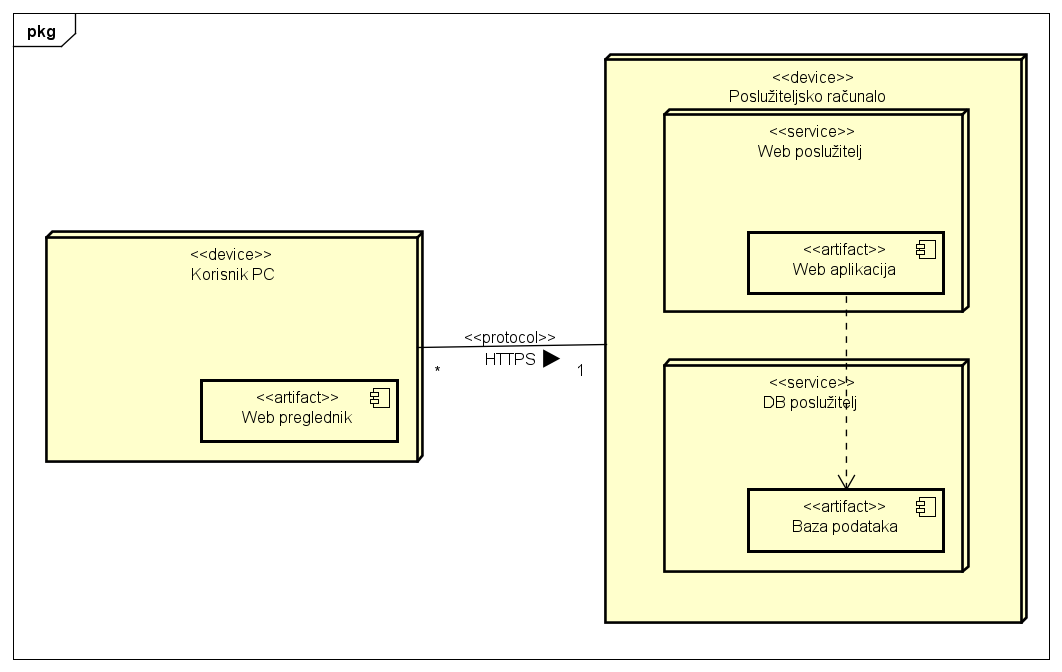
\includegraphics[width=\textwidth]{slike/DijagramRazmjestaja.png} %veličina u odnosu na širinu linije
				\caption{Dijagram Razmještaja}
				\label{fig:DijagramRazmještaja} %label mora biti drugaciji za svaku sliku
			\end{figure}
			
			\eject 
		
		\section{Upute za puštanje u pogon}
		
			\textbf{Instalacija poslužitelja baze podataka}\\
		
			 Potrebno je preuzeti Oracle MySql bazu podataka (za operacijski sustav Windows).
			 Poželjno je skinuti čitav paket Oracle Workbench. Nakon toga je potrebno provesti standardnu instalaciju s postavljanjem korisnika.
			
			
			 \textit{Dovršenu aplikaciju potrebno je pokrenuti na javno dostupnom poslužitelju. Studentima se preporuča korištenje neke od sljedećih besplatnih usluga: \href{https://aws.amazon.com/}{Amazon AWS}, \href{https://azure.microsoft.com/en-us/}{Microsoft Azure} ili \href{https://www.heroku.com/}{Heroku}. Mobilne aplikacije trebaju biti objavljene na F-Droid, Google Play ili Amazon App trgovini.}
			
			
			\eject 